\section{Prototype Development}

% ---------------------------------------------------------------------------------------------------------------------
\subsection{Evaluation-Driven Development: Formative Prototype Evaluation during Development}
\label{sec:evaluation-driven-development}

% --> neue Version hier:

Die Entwicklung des Prototyps folgte dem Evaluation-Driven Development (EDD) Ansatz (vgl.
\autoref{sec:evaluation-driven-development}). Dabei kamen bereits während der Implementierung automatisierte
Prüfverfahren zum Einsatz, um das System kontinuierlich zu evaluieren.

Nutzerstudien, Human-in-the-Loop-Evaluierungen oder Expertenbewertungen waren in dieser frühen Prototyping-
und Entwicklungsphase nicht praktikabel, da solche Verfahren ohne erheblichen Aufwand nicht skalierbar sind.
Stattdessen erfolgte die Weiterentwicklung des Systems in kurzen Zyklen aus Implementierung, Prüfung und
Anpassung. Dieses iterative Vorgehen ist in der Softwareentwicklung etabliert (vgl.
\cite[p.~8]{ottAppsEffektivManagen2019}) und besonders bei EDD von KI-basierter Systeme relevant, da aufgrund
der vielfältigen Nutzungsmöglichkeiten hier kein vollständiges Testorakel vorausgesetzt werden kann
\cite[p.~39]{istqbrISTQBCertifiedTester}.

Für Komponenten, die nicht auf probabilistische KI-Modellausgaben angewiesen waren, sowie Unit- und
Integrationstests, kamen klassische Softwaretests zum Einsatz, da sich für diese ein eindeutiges und
deterministisch prüfbares Testorakel definieren ließ. Da der überwiegende Teil des zu testenden Systems
jedoch auf LLM-basierte Komponenten angewiesen und somit probabilistisch ist, war dies in den meisten Fällen
nicht möglich.

Deshalb wurde ein von der Methode „LLM-as-a-Judge“ inspirierter Ansatz gewählt (vgl.
\autoref{sec:llm-as-a-judge}). In der hier verwendeten Version bewertete das LLM den Output nicht in
Echtzeit, sondern wurde genutzt um im Voraus Szenarien (meist mögliche Konversationen) für spezifische
Situationen zu generieren, um ein lexikalisches Testorakel zu erstellen. Dieses wurde im Rahmen
codebasierter (vgl. \autoref{sec:code-based-testing}) automatiserierter Test, in Kombination mit regulären
Ausdrücke verwendet.
Das vom LLM-Judge genereierte Orakel operationalisierte, welche Formulierungen eine fachlich angemessene
Facilitator-Äußerung in dem jeweiligen Szenario aufweisen muss und welche sie nicht aufweisen darf. Der Output
der einzelnen Komponenten wurde überwacht und analysiert, um das Verhalten der Komponenten in den
verschiedenen Szenarien besser verstehen und bewerten zu können.

Während der Entwicklung wurde das System kontinuierlich in unstrukturierten, explorativen Tests,
sowohl einzeln als auch unregelmäßig mit mehreren Personen in verschiedenen, nicht weiter spezifizierten
Szenarien überprüft. Ziel war es, bereits vor den eigentlichen Nutzerstudien (vgl.
\autoref{ch:empirical-prototype-validation}) ein Gefühl für das Systemverhalten zu entwickeln. Dadurch
sollten offensichtliche Fehler sowie kritische Schwachstellen, an denen das System vom intendierten
Verhalten abweicht, frühzeitig erkannt werden, um das System anzupassen.

Dieses Vorgehen kann in einem Loop wie folgt dargestellt werden:

\begin{figure}[H]
  \centering
  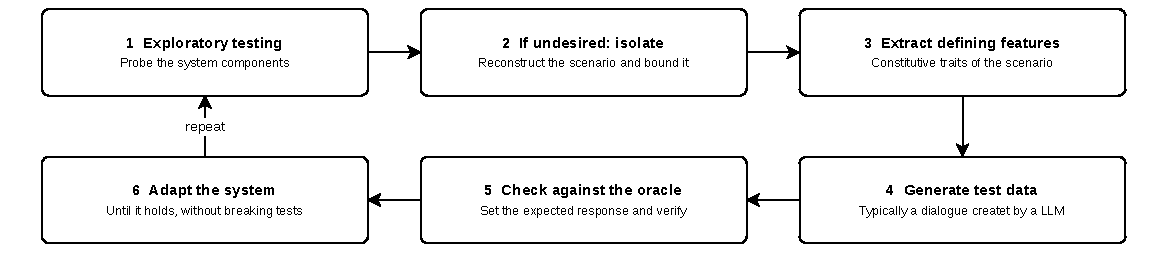
\includegraphics[width=\textwidth]{assets/figures/04/evaluation-driven-development-loop.pdf}
  \caption{Evaluation-driven development loop: From exploratory testing to system adaptation
  \figsource{Own illustration, created with draw.io.}}
  \label{fig:evaluation-driven-development-loop}
\end{figure}

Somit wurde nach und nach das Testorakel immergrößer, welches dann gleichzeitgt für regressionstest genutzt
werden konnte, um zu erkennen ob eine Systemänderung bereits getestete Szenarien negativ beeinflusst.
Die bestehenden Fälle fungierten damit als Regressionstests: Eine lokale Verbesserung durfte zuvor
gesichertes Verhalten nicht beeinträchtigen.

\minisec{Limitierungen des Vorgehens}
\label{sec:edd-limitations}

Ein lexikalisches Orakel ist unvollständig und die qualität hängt in diesem Fall von dem LLM-Judge ab.
Eine gültige Facilitator-Äußerung kann das intendierte Verhalten zeigen, ohne die vorgesehenen
Wortgruppen zu enthalten; umgekehrt kann ein Treffer formal korrekt und situativ unpassend sein.
Isolierte Dialoge blenden zudem die Dynamik eines echten Meetings aus: Turn-Taking, Timing und die
Reaktion der Gruppe auf eine Intervention bleiben unberücksichtigt.
Welche Szenarien überhaupt als Testdaten aufgenommen wurden, hängt außerdem von den explorativ
beobachteten Fehlern ab und ist damit autorenseitig selektiert.

Dennoch entspricht diese Kombination, von kontinuierliche, orakelgestützte Prüfung während der Implementierung und
unabhängige Human-in-the-Loop-Evaluation danach (druch die User Studien), einem valider Ansatz zum prüfen von
llm basierten agentischen Systemen.
\cite[pp.~6--7]{mohammadiEvaluationBenchmarkingLLM2025}.

% Während der Entwicklungsphase ist es unpraktisch, für jede Code-Änderung oder Anpassung von Parametern
% Nutzerstudien durchzuführen. Die Autoren von Inner Thoughts schlagen dafür eine Multi-Agenten-Simulation vor.
% \cite["6 Simulative Evaluation"]{liuProactiveConversationalAgents2025}
% Dabei wurden in diesem verschiedene Thoughtful Agents mit den unterschiedklciehn Infromationen und Profilen
% aus dem hidden-Profiles experiment ausgestattet, sodass der Gesprächsverlauf zwischen den KI-Agenten
% simuliert werden kann. Während der Entwicklung wird dabei
% ausschließlich die Moderationsstrategie des AI-Facilitators variiert bzw. optimiert.

% Es wirde die Einschätzung von Liu et al. geteilt, dass eine solche Simulation skalierbar ist und sich
% Fehler im Moderationsverhalten (z.B. unpassendes Timing oder Unterbrechungen) über längere Interaktionen
% hinweg akkumulieren und verstärken \cite["6 Simulative Evaluation"]{liuProactiveConversationalAgents2025}.
% Ein schlechtes Systemdesign, ungeeignete Prompts oder Parameter sollten demnach zu einer erkennbar
% schlechteren Gesprächsqualität führen.

% Für die Evaluierung der Gesprächs- bzw. Moderationsqualität käme ein menschlicher Bewerter in Form von
% Facilitating-Experten infrage.
% Da das ausgewählte Hidden-Profile-Verfahren jedoch etwa 30 Minuten dauert, ist dies während der
% Entwicklungsphase kaum praktikabel, weil die Aussagekraft der Evaluierung mit jeder weiteren Anpassung des
% Systems abnimmt und die Systemausgaben nach jeder Modifikation erneut aufwändig bewertet werden müssten.

% Aus diesem Grund wurde ein LLM-as-a-Judge-Ansatz mit einer G-Eval-Replikation gewählt, der die allgemeine
% Meetingqualität basierend auf dem Fragebogen von XY abgeleitetn Kriteren bewerten sollte.

% Zusätzlich evaluierte ein weiteres LLM, ob die Teilnehmer alle relevanten Informationen von den Steckbriefen
% genannt hatten. Diese Klassifizierung wurde anschließend statistisch ausgewertet.

% Darüber hinaus wurden mithilfe von LLMs Gesprächsszenarien systematisch generiert, in denen ein Facilitator
% eingreifen würde. Ziel war es, das "External Stimulus Injection Layer" zu überprüfen. Dabei wurde analysiert,
% wie häufig der AI-Facilitator an den erwarteten Stellen aufgrund des gesetzten External Stimulus eingriff.
% Diese automatisierten Tests wurden während des Systemdesigns und der Entwicklung regelmäßig durchgeführt,
% sobald der Autor eine Änderung vorgenommen hatte, von der er sich eine Verbesserung erhoffte.

% Somit wurde versucht sich bassierend auf diesen Tests zu qualifizieren ob die Entwicklung eines Moderation
% System in eine Richtung geht, die die Qualität des Meetings in einer hiddenprofile konstelation verbessert.

% Um die aussagekraft in realen Bedinung mit Menschen zu evaluieren wurden nach der Entiwkclungsphase
% Usability-Studien durchgeführt.
% (vgl. Section XYZ TODO)

% ---------------------------------------------------------------------------------------------------------------------
\subsection{System Architecture: Adapted version of the “Inner Thoughts” framework}
\label{sec:adapted-inner-thoughts}

\begin{figure}[H]
  \centering
  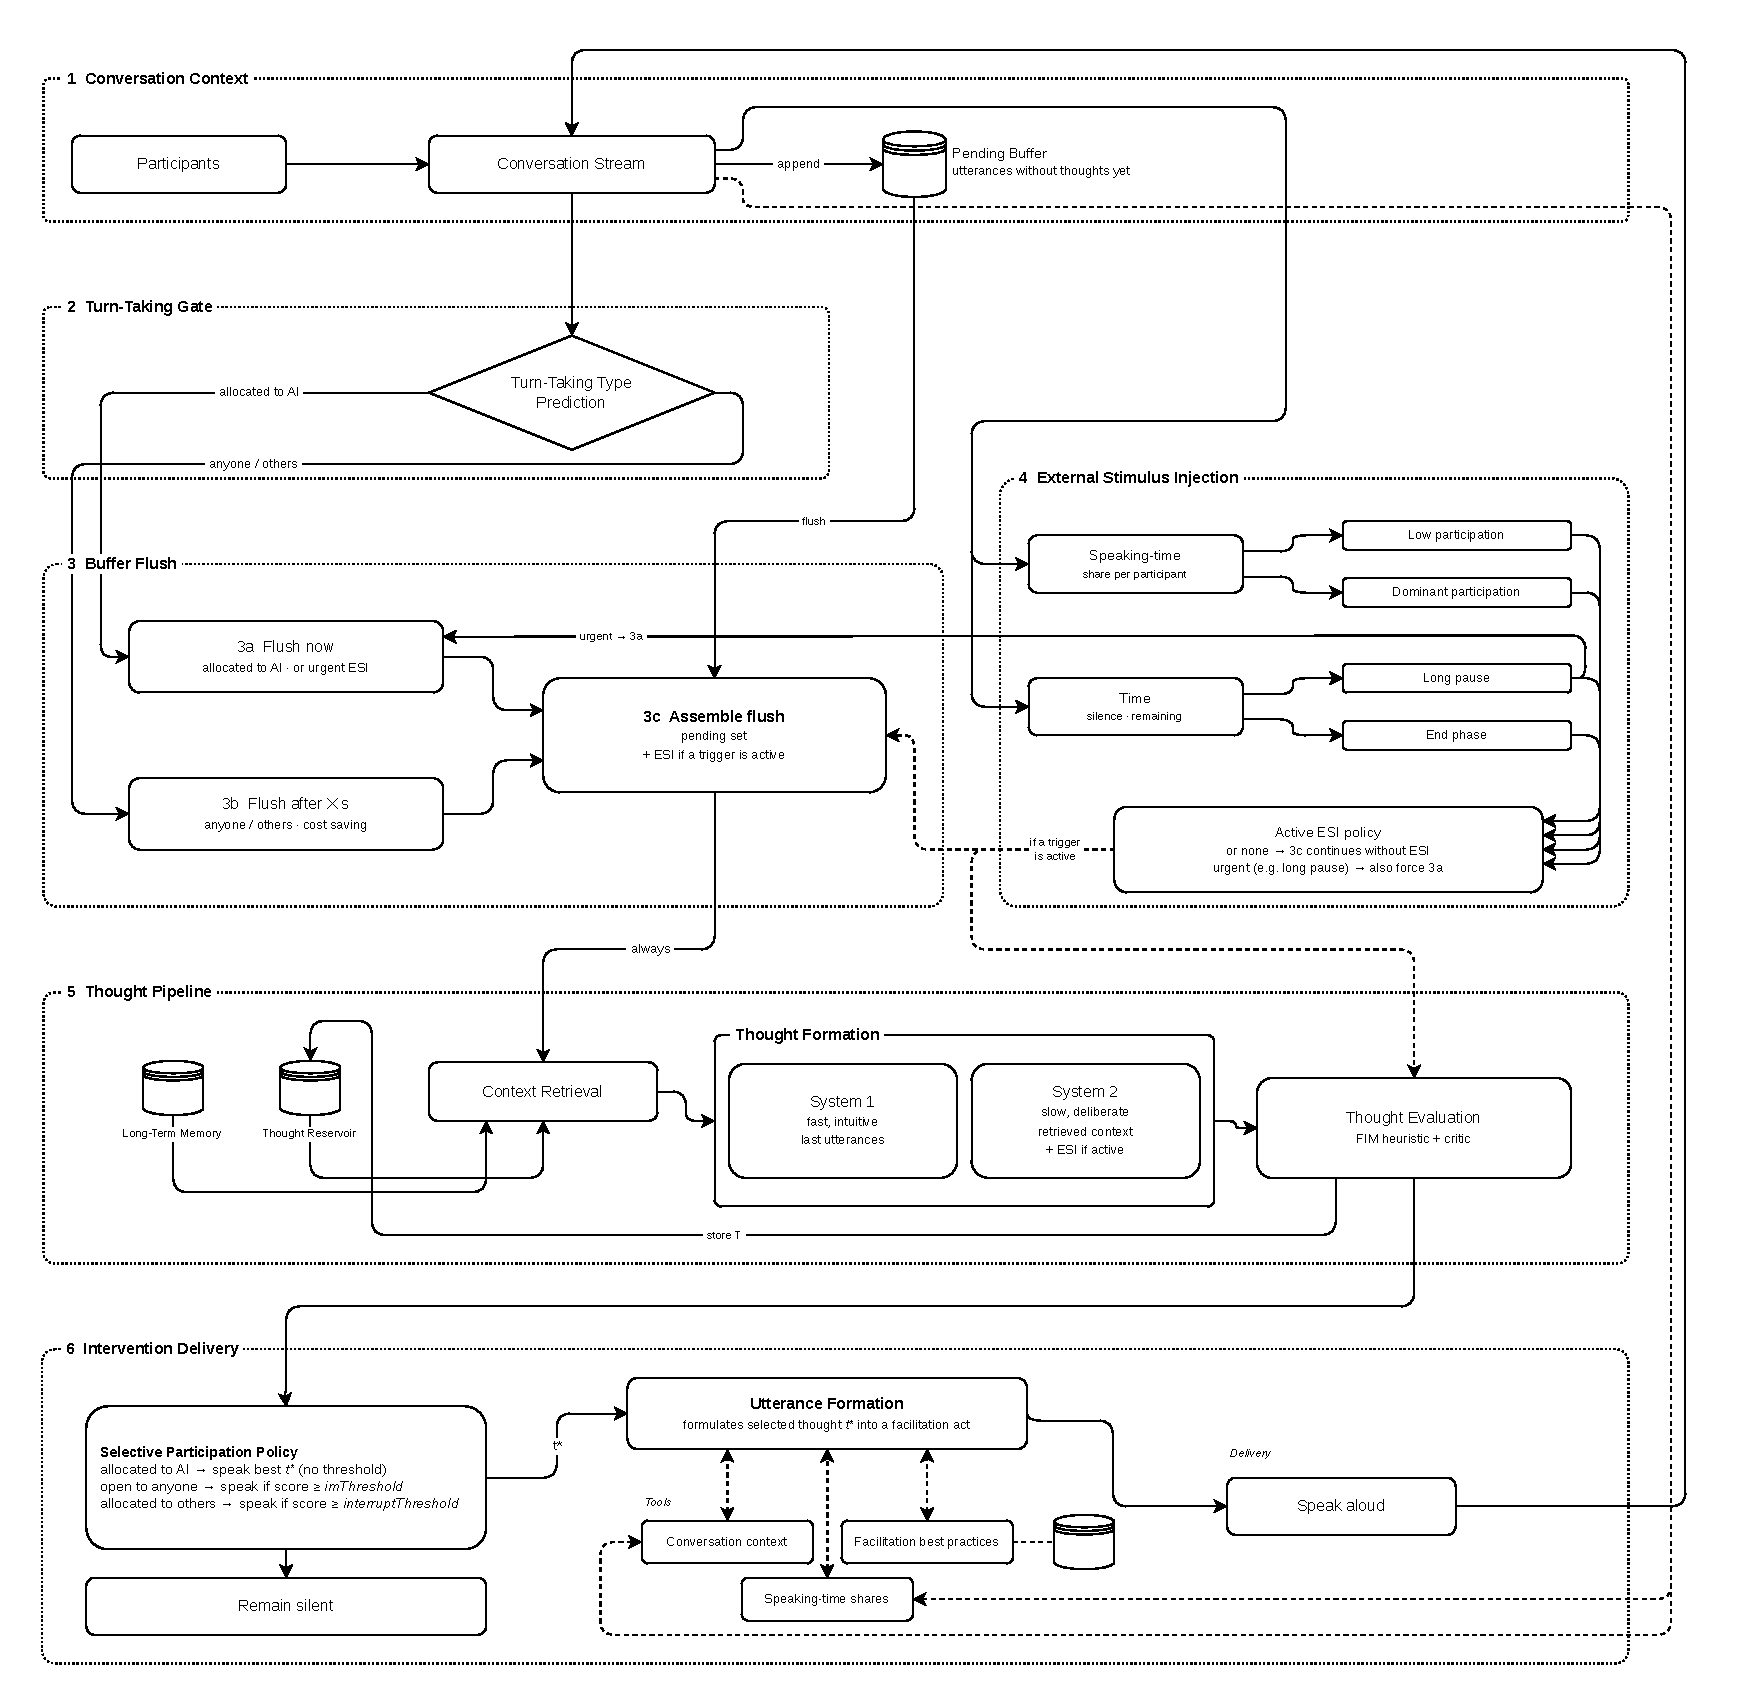
\includegraphics[width=0.99\textwidth]{assets/figures/04/system-architecture.pdf}
  \caption{System Architecture: Adapted version of the “Inner Thoughts” framework
    \figsource{Own illustration based on "Inner Thoughts" by Liu et
  al.\cite{liuProactiveConversationalAgents2025}, created with draw.io.}}
  \label{fig:system-architecture}
\end{figure}

\begin{figure}[H]
  \centering
  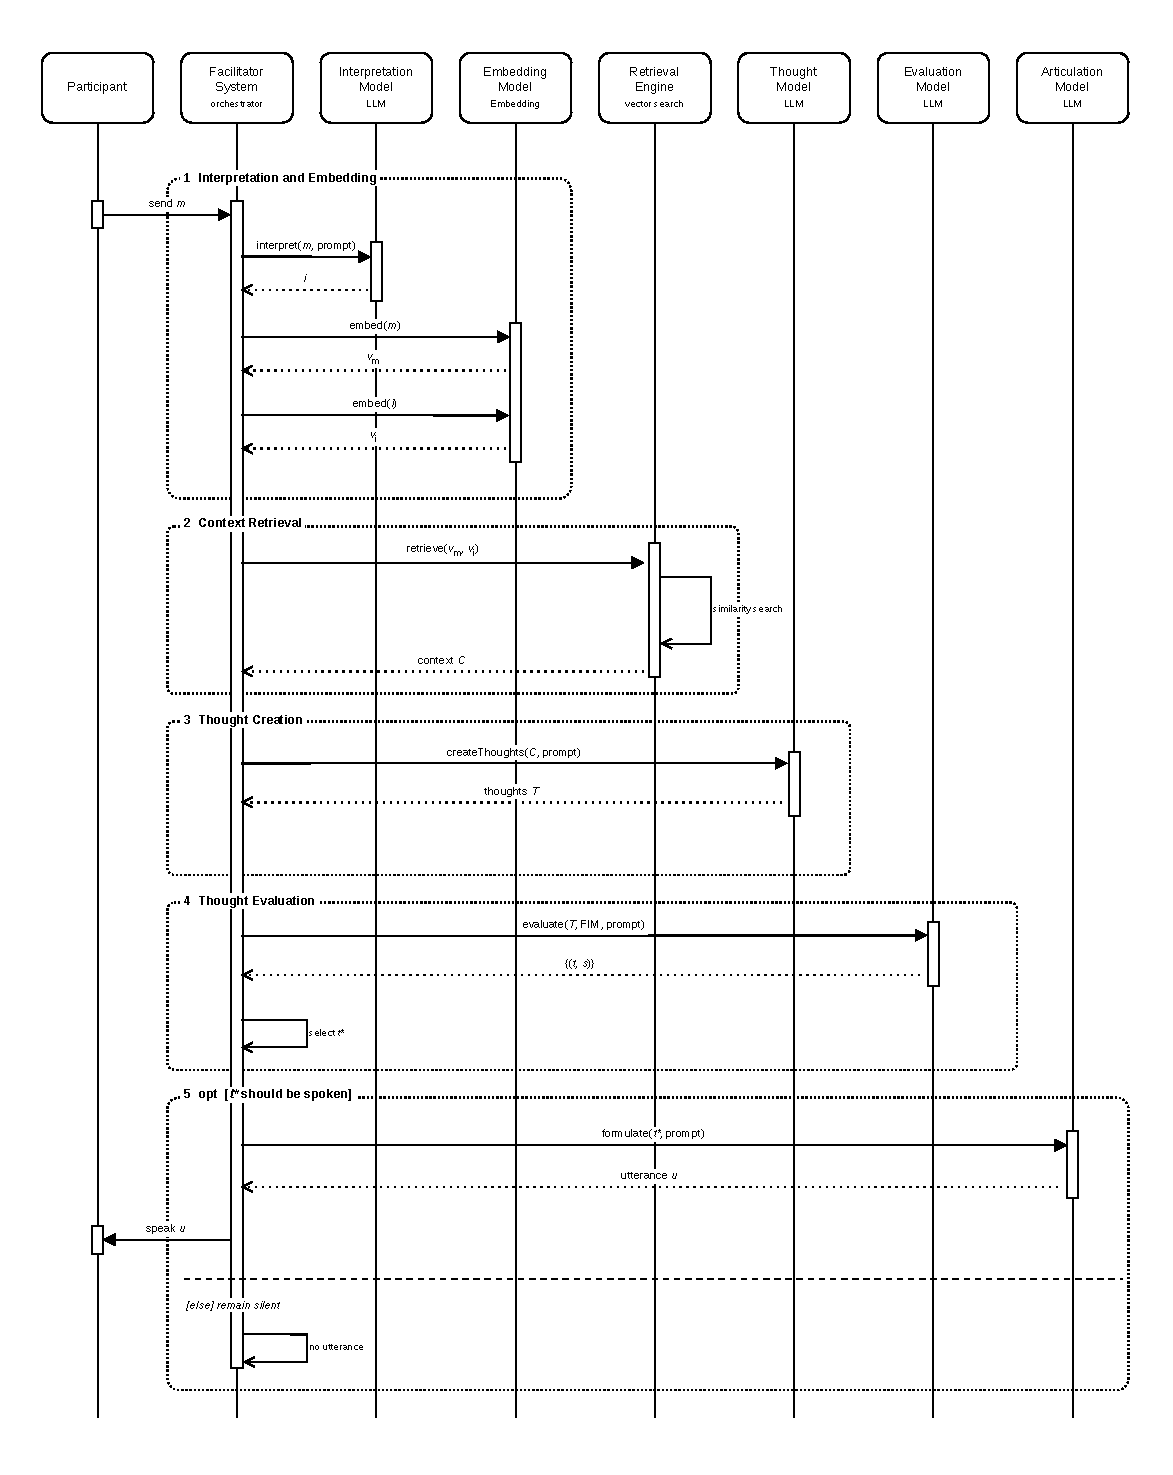
\includegraphics[width=0.97\textwidth]{assets/figures/04/thought-pipeline-sequence.pdf}
  \caption{Thought Pipeline Sequence: Sequence of the thought pipeline
    \figsource{Own illustration based on "Inner Thoughts" by Liu et
  al.\cite{liuProactiveConversationalAgents2025}, created with draw.io.}}
  \label{fig:thought-pipeline-sequence}
\end{figure}

Das Inner Thoughts- Freamwork von Liu et al. ist in deren version eher für interaktionen ausgelegt die als
soziales Plaudern kotegorisertet werden können. Dies ist nicht was ein Faciliator machen würde. Die Idee ein
KI-System anhand einer intrsisichen motivation zu modellieren, bevor jemand etwas zu einer Gruppen discussion
beiträgt, ist dennoch auch für diese ARbeit relevant.
Insbesondere weil dieser Ansatz darauf hindeutet eine erhöhte Genauigkeit bei self-trun-allocation zu erzeugen.
Aus den Experten ging hervor ds eine Geanken gänge, welche Facilitatoren haben auf abstakter inutionen
basieren andere wiederum druchdacht kombiniert mit experten wissen etc. Dies legt nach,
dass legt nahe das sowhl system 1 als auch system 2 bei dem prozess involoviert sind, was eben falls in dem
Innter Thougs Framewokr berücksichtigt wird.

Die Autoren wiesen in der Diskussion der Arbeit \cite["8.2 Apllying Inner Thougs Beyond Casual
Conversations"]{liuProactiveConversationalAgents2025} selbst darauf hin, dass sich das System durch anpassungen der
Bewertungskriterien auf aufgabenorietnerte Kontexte anpassen lässt und zielorientiertes praktives Handeln
ermöglichen kann. Sie schalgen vor für weitere arbieten das system mit domain-specifische heuristiken
anzupassen, um die interaktionen an real-world tasks zu orientieren.

Im ursprünglichen Modell von Liu et al. werden generierte Gedanken primär danach bewertet, wie stark sie die
"persönliche Relevanz" die individuellen Interessen oder die einzigartigen persönlichen Kenntnisse des
Agenten widerspiegeln (TODO: prüfen bzw. konkretisieren wie die heuristik tatsächlich ist). Dies mag für
generische Conversationen geeigent sein, da dieser Ansatz Authentizität und
Sympathie in infromellen, sozialen Unterhaltungen erhöht, ist für einen AI-Moderator in zielorientierne
Meetings die durch Hidden Profile geprägt sind, allerdings ungeeiengt. Wenn die Gedanken des AI-Moderator
primär danach bewertet würden, wie stark sie seinen "persönlichen Interssen" wiederspieglen, verfällt er in
dassaelber fehlerhafte Verahltensmuster, das zu verzeruung in hidden profile situationen führen kann. Er
bringt eingen Meinungen oder Präferzene ein statt die diskussion neutral zu strukturieren. Strukturelle
prozeduelle Gedanken würde in der aktuellen Heurisik voraussichtlich mit zu niederiger Relevanz bewertet werden.

Bei der Anpassung der Heurisitken und prompts wurden sowohl die Literatur als auch die erkentnisse aus den
Interviews berücksichtigt. Die Evaluierungs-Heursitik zu bewertung der Gedanken wurde so angepasst, dass sie
das kognitionspyschologsche Fundament des Innter Thoughts-Modelles (basierend  auf grice, Sacks, Goffman und
Berly) mit en organisationspsychologischen Prinzipien zur Kompenstation des Shared Information bias (Stasser \&
Titus; Brodbeck et al.) und den HCI-Richtlinen für inklusive Moderation (Houttie et al; Davison) kombiniert.

In der original Modellering des Inner Thougs-Frameworks wird ide participation in einer kovversation
ausschlielich basierend der innern gedanken abgeleitet. Die Authoern mekren an, dass exteren Cues nicht im
ausschleiieß zu ihrer Methode stehen sondern complentär mit exteren cues kombiniert zu einem robustern system
führen könnten. \cite[8.1 Proactive Agents via Intrinsic Motivation vs. Extrinsic
Cues]{liuProactiveConversationalAgents2025}

Eine kernproblematik bei hidden profies ist, das private inforamtione nicht getielt werden. Ein indikator
dafür könnte sein, dass eine person sich an der converstation nicht beteiligt oder ander Teilnehmden die
Diskussion domieren, so dass andere nicht zu wort kommen können. wie aus den interviews
hervorging, würde ein facilitator hier typischer weise versuchen diese Person auf höfliche art zu integrieen,
um deren Perspektive zu hören. Hierfür wäre extern Cues wie die Sprrecheranteile relevant. Um diese
exteren Cues abzubilden wurde das Inner Thoughs Framework, um die Komponete "External Stimulus Injection" erweitert.
Ist einer dieser externe Trigger erfüllt wird ein vordefinierter Gedanke in der Gedanken generierung von
System 2 berügcksichtig und die Evaluations herusitik bewsust in richtung diesen extern Triggers gebaiased,
um zu erzielen dass diese externe cue im innerthoughs modeel gewichtet wird.

%%%%%%%%%
Baseirend auf der Literatur und den Intervies wurde versucht dieses System entpsrechend zu adaptieren.

Ein prblem ist die tendenz von KI zu überkompensieren und zu viel zu sagen. Die authoren merken dies auch an
und sind optimistischen, dasss ihr conversational agent hier besser performt. Alelrdigns handelt es sich um
eine plausch. Ein facilitator würde nicht so oft in die Diskussion eingreifen. Das risiko für
overcompensationg mit diesem system ist hoch. mit dem imThreshold kann gesteuert werden wie schwerwwiegend
ein Gedanke sein muss damit die KI ihn überhaupt aussproche.

In dem Paper wurd ein Selective Participant modeliert, welche foglende Parameter hatte:

- System1 wurde auf 0 gesetzt so das die KI also niemals äußert niemals spontane, ungeplante
System-1-Floskeln äußert. Jeder Beitrag muss einen teifen, kognitiven Nutzen haben.
-imThreshold wurde auf 4.3 gesetzt. Ein strategeischer Gedanke muss auf einer Skala von 1-5 einen extrem
hohe Bewertung erreichen, um die schwelle zu reißen. Ein einfacher Gedanke wie "ICh könnte Bob mal wieder
fragen" reicht dafür nicht aus. Es bedarf eines
Phase 1 Trigger:

% ---------------------------------------------------------------------------------------------------------------------
\subsection{Components: Transcription, Analysis, and Intervention Modules}

Abgleeite aus dem Paper Keeper. Der Agent könnte auch eine visualle Warteschlage steuern. anstatt aktiv zu
unterbrechen sezt ersich auf die warteschalge bzw. hebt die hand, um sich anzukündigen.
% Wenn dein AI-Facilitator interveniert, um den Shared Information Bias zu brechen, muss er dies nicht zwingend
% über eine störende, verbale Unterbrechung tun. Du kannst vorschlagen, dass der Agent eine visuelle
% Warteschlange steuert (z. B. "Ich setze Bob als nächsten auf die Rednerliste, da er zu Kriterium X wertvolle
% ungeteilte Infos hat"). Das senkt die kognitive Last der Teilnehmer und sichert ihre Aufmerksamkeit.

\textbf{FIM-Heuristik}

\textbf{Thought-Evaluation}

The full FIM scoring prompt, with a unit-by-unit provenance relative to the
original Inner Thoughts evaluation protocol, is documented in
\autoref{annex:fim-scoring}.

Angelengt an die Thoguht Evaluation Phase von XX (procativ Conversation Agents) wurde auch in diesem sich dem
contextual self-refinement bedient.
Self-Refinement und Reflexion könnnen bei LLMs zu drastischen ELsitugssteirgunen führen, wenn eine kognitive
Feedbackschleife druchaufen wird. \cite[p. 18]{meiSurveyContextEngineering2025} Ein Gedanke wird nicht direkt
ausgesprochen, sondern druch einen Kritiker basierend auf der für diese arbeit entwicklete FIM-Heurisitk geprüft.
The evaluation protocol follows the G-Eval prompt structure \cite[p. 2512]{liuGEvalNLGEvaluation2023}
similarly also used for Thoughtful Agents. Probability-weighted scoring as proposed in the original method
was omitted as a pragmatic decision, because the APIs used here do not return output-token probabilities.

In practice every utterance is appended to a shared pending buffer of messages that have not yet
been thought about. The turn-taking prediction only decides \emph{when} that buffer is flushed
(immediately if the floor is allocated to the AI; otherwise after $X$ seconds as one batch). Both
cases continue to the same next step: the flushed pending set is assembled and the thought pipeline
runs. External Stimulus Injection is not a later stage. Its monitors run continuously, but an ESI
policy joins the pipeline only at that flush, and only if a trigger is active; otherwise the
pipeline runs without it. A selected thought $t^{*}$ is not spoken raw. An Utterance Formation
agent formulates it into a facilitation act, with tools for conversation context, facilitation best
practices, speaking-time shares, sending a chat message, or speaking aloud.
The articulation prompt and the mapping from the original Inner Thoughts
wording are documented in \autoref{annex:articulation-prompt}.

\autoref{tab:architecture-design-decisions} maps each architectural choice to a single warrant and to the
chapters that already establish it, so the implementation can be traced without restating those arguments.
\clearpage
\begin{table}[H]
  \centering
  \caption{Architectural design decisions of the adapted Inner Thoughts prototype, with rationale and
  pointers to the motivating chapters of this thesis.}
  \label{tab:architecture-design-decisions}
  \small
  \setlength{\tabcolsep}{4pt}
  \begin{tabularx}{\textwidth}{@{}
      >{\raggedright\arraybackslash}p{2.85cm}
      >{\raggedright\arraybackslash}X
      >{\raggedright\arraybackslash}p{3.55cm}
    @{}}
    \toprule
    \textbf{Design decision} & \textbf{Rationale} & \textbf{Evidence} \\
    \midrule
    Adapt Inner Thoughts from casual talk to facilitation
    & The original model times utterances by intrinsic motivation, which improves self-turn-allocation
    in multi-party talk. Liu et~al.\ already invite domain-specific evaluation criteria for
    goal-directed settings; without that shift, a facilitator would be scored as a social
    conversationalist.
    & \autoref{sec:proactive-ai-interactions} \\
    \addlinespace
    Replace personal-relevance scoring with a facilitation-oriented FIM heuristic
    & Ranking thoughts by the agent's own interests would privilege preference talk, undervalue
    procedural structure, and reproduce the shared-information bias the moderator is meant to
    counteract.
    & \autoref{sec:hidden-profiles};
    \autoref{ch:empirical-analysis-of-facilitating-strategies} \\
    \addlinespace
    Inject external participation cues into thought generation
    & Unique information stays private when speakers remain silent or are crowded out. Observable
    speaking-time imbalance is a complementary cue, not a rival, to intrinsic motivation; expert
    facilitators report inviting quiet members rather than waiting for self-selection.
    & \autoref{sec:hidden-profiles};
    \autoref{sec:key-challenges-in-meetings};
    \autoref{ch:empirical-analysis-of-facilitating-strategies} \\
    \addlinespace
    Selective-participant policy: no System-1 speech, high \textit{imThreshold}
    & Facilitation needs sparse, high-utility interventions. Unconstrained generation over-talks;
    disabling System-1 filler and raising the utterance threshold admits only thoughts with clear
    process value.
    & \autoref{sec:facilitation};
    \autoref{sec:interaction-paradigms} \\
    \addlinespace
    Critic-based self-refinement before any utterance
    & A thought is spoken only after a critic applies the FIM heuristic. Contextual self-refinement
    implements an evaluator--optimizer loop and is associated with substantial quality gains in
    LLM pipelines.
    & \autoref{sec:context-engineering};
    \autoref{sec:ai-agent-building-blocks} \\
    \addlinespace
    Cheap temporal reweighting instead of LLM re-scoring
    & Static IM speaks stale thoughts. Re-prompting every thought after each event is too slow and
    costly for a live meeting. Linear aging and a post-speech smoothstep keep the original score
    but discount age and repetition.
    & \autoref{sec:adapted-inner-thoughts} \\
    \bottomrule
  \end{tabularx}
\end{table}
\FloatBarrier

\minisec{Dynamic intrinsic motivation}
\label{sec:dynamic-im}

In the original Inner Thoughts model, intrinsic motivation is static: a thought is scored once at
generation and that score never changes. Early tests during development showed that the system spoke thoughts
that the subsequent discussion had already made obsolete, and that would, if they would have been evaluated
again, probably no longer would have received a high FIM score given how the meeting had evolved.

% TODO: beispielhafter Chatverlauf, in dem ein statischer FIM-Score zu spät geäußert wird.

Re-scoring every pending thought with an LLM after each event would restore recency, but the added
latency and cost would make the system unusable in a live meeting. The prototype therefore keeps the
original FIM score and applies a cheap, deterministic reweighting under two assumptions:
\begin{itemize}
  \item A facilitation thought becomes a poorer description of the current state and process need as the
    conversation moves on, because later information was not available when it was scored.
    As the meeting continues, the group may already have closed that gap, a quiet participant may have
    spoken, unique information may have surfaced, or the discussion may have moved on.
    Therefore its priority should fall with age.
  \item Once a facilitation intervention has been spoken, repeating it immediately could result in over-talking and
    crowd the discussion. The motivation to raise the same process issue is therefore initially very low, but
    may recover if the group still does not take it up.
\end{itemize}

Let \(S=[1,5]\) be the FIM scale, \(T=[0,\infty)\) elapsed time in seconds, and
\(T_{\infty}=[0,\infty]\) time since last speech, where \(\infty\) means never spoken.
To each triple \((s_0,t,t_{\mathrm{spk}})\in S\times T\times T_{\infty}\) the mapping
\(s_{\mathrm{weighted}}\) assigns one weighted score. Aging and cooldown address the two
assumptions (see above), so they are modeled as a product:

\begin{equation}
  s_{\mathrm{weighted}} :
  \begin{cases}
    S \times T \times T_{\infty} \to [0,5] \\
    (s_0,\, t,\, t_{\mathrm{spk}})
    \mapsto
    \min\bigl(5,\, \max(0,\, s_{\mathrm{aged}}(s_0,t)\cdot c(t_{\mathrm{spk}}))\bigr).
  \end{cases}
  \label{eq:im-weighted}
\end{equation}

The session-wide parameters \(\tau\), \((s_{\mathrm{hold}}, t_{\mathrm{hold}})\) and
\(t_{\mathrm{cool}}\) determine the kernels \(s_{\mathrm{aged}}\) and \(c\) below.

\paragraph{Aging \(s_{\mathrm{aged}}\).}
Later information was not available when the thought was scored, so priority falls with age.
Linear decay hits zero at a finite horizon \(H\):

\begin{equation}
  s_{\mathrm{aged}} :
  \begin{cases}
    S \times T \to [0,5] \\
    (s_0,\, t) \mapsto \max\bigl(0,\, s_0(1-t/H)\bigr).
  \end{cases}
  \label{eq:im-aged}
\end{equation}

Linear decay is a practical modelling assumption: it is simple and reaches zero in finite time
(\autoref{fig:im-aging}). \eqref{eq:im-aged} is the straight line from \((0,s_0)\) to \((H,0)\),
hence of slope \(-s_0/H\).

The horizon \(H\) is not chosen directly. A thought of score \(s_{\mathrm{hold}}\) should remain
above \(\tau\) for \(t_{\mathrm{hold}}\) seconds, so that line must pass through
\((t_{\mathrm{hold}},\tau)\). Equating the two expressions for the slope and solving for \(H\)
gives
\begin{equation}
  \begin{aligned}
    -\frac{s_{\mathrm{hold}}}{H}
    &= \frac{\tau-s_{\mathrm{hold}}}{t_{\mathrm{hold}}}, \\[0.35em]
    H
    &= \frac{t_{\mathrm{hold}}}{1-\tau/s_{\mathrm{hold}}}.
  \end{aligned}
  \label{eq:im-horizon}
\end{equation}

All thoughts share this \(H\). A weaker thought therefore crosses \(\tau\) sooner. The pair
\((s_{\mathrm{hold}}, t_{\mathrm{hold}})\) is the only design knob for temporal sensitivity: a
shorter \(t_{\mathrm{hold}}\) steepens every line (\autoref{fig:im-aging}).

\begin{figure}[H]
  \centering
  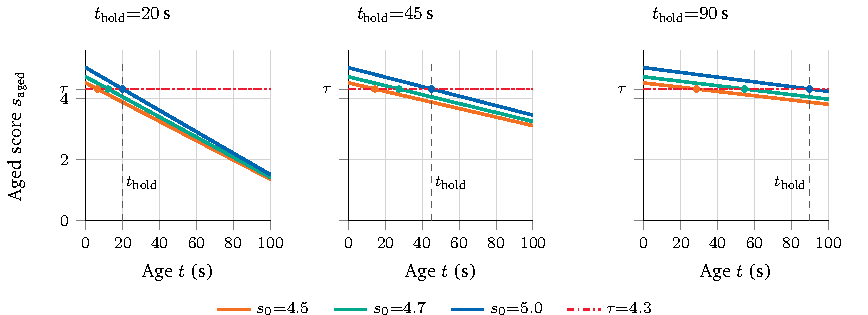
\includegraphics[width=\textwidth]{assets/figures/04/im-aging.pdf}
  \caption{Linear aging of the FIM score at three hold-times. Each panel shows the same
    scores \(s_0\in\{4.5,4.7,5.0\}\); the vertical line is \(t_{\mathrm{hold}}\), where a
    score-5 thought crosses \(\tau\). Within a panel, weaker thoughts expire sooner. Left to
    right, a shorter \(t_{\mathrm{hold}}\) steepens every line.
    Parameters: \(\tau=4.3\), \(s_{\mathrm{hold}}=5\).
  \figsource{Own illustration, created with LaTeX and TikZ}}
  \label{fig:im-aging}
\end{figure}

\paragraph{Cooldown \(c\).}
Once spoken, the motivation to repeat a facilitation intervention is initially very low, but may
recover if the group still does not take the process issue up.

\begin{equation}
  c :
  \begin{cases}
    T_{\infty} \to [0,1] \\
    t_{\mathrm{spk}} \mapsto \mathrm{smoothstep}(t_{\mathrm{spk}}/t_{\mathrm{cool}}),
  \end{cases}
  \qquad
  \mathrm{smoothstep}(x)=
  \begin{cases}
    0 & x\le 0,\\
    3x^{2}-2x^{3} & 0<x<1,\\
    1 & x\ge 1.
  \end{cases}
  \label{eq:im-smoothstep}
\end{equation}

For \(t_{\mathrm{spk}}=\infty\) the quotient is \(\infty\), hence \(c(\infty)=1\).

The cubic \(3x^{2}-2x^{3}\) is the Hermite interpolant on \([0,1]\) with vanishing endpoint
derivatives, chosen so that recovery pauses after speech and returns to 1 without a hard knee
(\autoref{fig:im-cooldown}).

\begin{figure}[H]
  \centering
  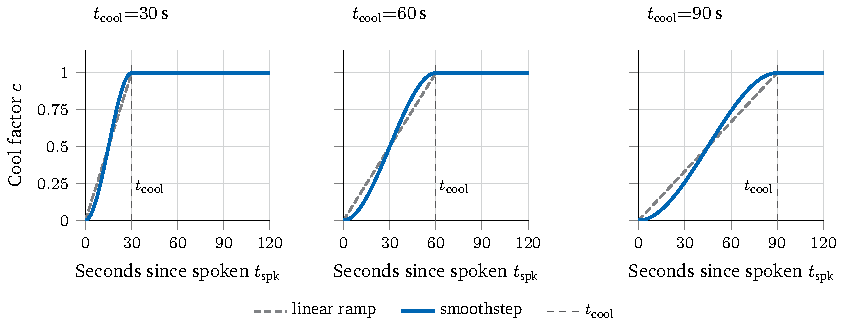
\includegraphics[width=\textwidth]{assets/figures/04/im-cooldown.pdf}
  \caption{Cooldown factor after a thought is spoken, for \(t_{\mathrm{cool}}\in\{30,60,90\}\,\mathrm{s}\).
    Each panel compares the Hermite smoothstep with a linear ramp; the vertical line is
    \(t_{\mathrm{cool}}\), where recovery completes. The smoothstep stays flat at both ends;
    the linear ramp starts immediately and kinks at \(t_{\mathrm{cool}}\).
  \figsource{Own illustration, created with LaTeX and TikZ}}
  \label{fig:im-cooldown}
\end{figure}

The product in \eqref{eq:im-weighted} is the result (\autoref{fig:im-weighted}). A just-spoken thought
cannot be repeated. After \(t_{\mathrm{cool}}\) it may become eligible again, but only if
\(s_{\mathrm{aged}}\) is still above \(\tau\).

\begin{figure}[H]
  \centering
  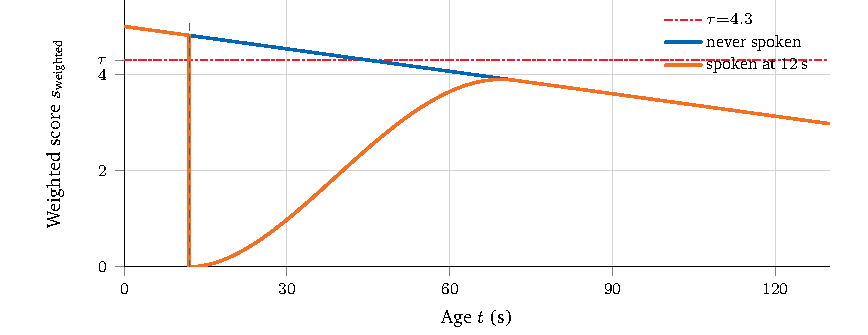
\includegraphics[width=\textwidth]{assets/figures/04/im-weighted.pdf}
  \caption{Weighted FIM score of a thought with \(s_0=5\), never spoken versus spoken at
    \(t=12\,\mathrm{s}\). Aging uses \(t_{\mathrm{hold}}=45\,\mathrm{s}\); cooldown uses
    \(t_{\mathrm{cool}}=60\,\mathrm{s}\). Recovery restores the aged remainder; whether that
    remainder still exceeds \(\tau\) depends on how long the thought has already lived.
    Parameters: \(\tau=4.3\), \(s_{\mathrm{hold}}=5\).
  \figsource{Own illustration, created with LaTeX and TikZ}}
  \label{fig:im-weighted}
\end{figure}

\minisec{Participation Balancer}
\label{sec:participation-balancer}

The Participation Balancer operationalizes \usref{us:quiet-voices} as two
speaking-time cues: curtailment of a dominant speaker and invitation of a
low-participation participant.
Unshared information in a hidden profile is introduced only by the participant who
holds it, and speaking turns are unequally distributed by status, with
higher-status participants intervening more frequently
(\autoref{sec:hidden-profiles}; \autoref{sec:key-challenges-in-meetings};
\cite{stasserExpertRolesInformation1995,bakerEnhancingGroupDecision2010,chenAreWeTrack2025,DoodleStateMeetings2019}).
Curtailment is therefore conditioned on a high individual share together with
another participant below half a fair slot, whereas invitation depends only on low
share and prolonged silence.

Let \(L>0\) be the planned meeting length and \(P\) the set of participants, with \(n=\lvert P\rvert\ge 1\).
Each participant's fair slot is
\begin{equation}
  F = L / n.
  \label{eq:fair-slot}
\end{equation}
Let \(r_i\ge 0\) be the speaking time participant \(i\) has accumulated, and let
\(i_{\star}\in P\cup\{\bot\}\) be the participant who currently holds the floor, or \(\bot\) if
nobody is speaking. Let \(\Delta_i\ge 0\) be the time since \(i\) last spoke, counted from the
start of the meeting if \(i\) has not spoken. The factor \(p>0\) is configured.

The current speaker is curtailed once their speaking time reaches \(p\) fair slots and at least
one other participant is still below half a fair slot:
\begin{equation}
  \mathrm{curtail}(i)
  \iff
  i = i_{\star}
  \;\land\;
  r_i \ge p \cdot F
  \;\land\;
  \exists\, j \in P\setminus\{i\}:\ r_j < F/2.
  \label{eq:balancer-curtail}
\end{equation}

Invitation uses two configured thresholds. \(\theta_r>0\) is the speaking time below which a
participant still counts as low-participation, and \(\theta_{\Delta}>0\) is the minimum time they
must have been silent since they last spoke. A participant is invited in when their own
speaking time is still below \(\theta_r\), they have been silent for at least \(\theta_{\Delta}\),
and they do not hold the floor:
\begin{equation}
  \mathrm{integrate}(i)
  \iff
  r_i < \theta_r
  \;\land\;
  \Delta_i \ge \theta_{\Delta}
  \;\land\;
  i \neq i_{\star}.
  \label{eq:balancer-integrate}
\end{equation}

% ---------------------------------------------------------------------------------------------------------------------
\subsection{Technology Stack: Facilitation Agent Runtime and Meeting Client}

Für die Entwicklung des AI-Facilitators wurden LangChain und LangGraph als zentrale Frameworks ausgewählt.
LangChain bietet eine modular aufgebaute Toolbox für die effiziente Entwicklung von LLM-basierten
Anwendungen, während LangGraph die Definition und Steuerung agentenbasierter Workflows ermöglicht.

Für die Durchführung der User Study wurde eine eigens entwickelte Webanwendung eingesetzt, die als einfache
Videokonferenzlösung fungiert. Diese wurde mit Svelte, SvelteKit und Tailwind CSS implementiert und auf einem
Hetzner-Server gehostet. Teilnehmer:innen konnten über einen teilbaren Link direkt auf die Anwendung zugreifen.
Der gewählte Ansatz ermöglichte eine direkte Analyse der Nutzerinteraktionen sowie eine optimierte User
Experience (UX). Alternativ hätte die Integration über bestehende Videokonferenz-Tools (z. B. als Bot via
API) in Betracht gezogen werden können. Allerdings wäre dies mit den Limitierungen der jeweiligen APIs
verbunden gewesen und hätte den Lösungsraum von vornherein eingeschränkt.
